%!TEX program = xelatex

\documentclass[compress]{beamer}
%--------------------------------------------------------------------------
% Common packages
%--------------------------------------------------------------------------

\definecolor{links}{HTML}{663000}
\hypersetup{colorlinks,linkcolor=,urlcolor=links}

\usepackage[english]{babel}
\usepackage{pgfpages} % required for notes on second screen
\usepackage{graphicx}

\usepackage{multicol}

\usepackage{tabularx,ragged2e}
\usepackage{booktabs}

\setlength{\emergencystretch}{3em}  % prevent overfull lines

\usetheme{hri}
\usetikzlibrary{shapes.geometric}
\usetikzlibrary{svg.path}

% Display the navigation bullet even without subsections
\usepackage{remreset}% tiny package containing just the \@removefromreset command
\makeatletter
\@removefromreset{subsection}{section}
\makeatother
\setcounter{subsection}{1}

\makeatletter
\let\beamer@writeslidentry@miniframeson=\beamer@writeslidentry
\def\beamer@writeslidentry@miniframesoff{%
  \expandafter\beamer@ifempty\expandafter{\beamer@framestartpage}{}% does not happen normally
  {%else
    % removed \addtocontents commands
    \clearpage\beamer@notesactions%
  }
}
\newcommand*{\miniframeson}{\let\beamer@writeslidentry=\beamer@writeslidentry@miniframeson}
\newcommand*{\miniframesoff}{\let\beamer@writeslidentry=\beamer@writeslidentry@miniframesoff}
\makeatother



\newcommand{\source}[2]{{\tiny\it Source: \href{#1}{#2}}}

\usepackage{tikz}
\usetikzlibrary{mindmap,backgrounds,positioning,calc,patterns}

\graphicspath{{figs/face_recognition/}{figs/}}

\title{Human-Robot Interaction}
\subtitle{Social Signal Processing}
\date{}
\author{Séverin Lemaignan}
\institute{{\bf Bristol Robotics Lab}\\University of the West of England}

\begin{document}

\miniframesoff

\licenseframe{github.com/severin-lemaignan/lecture-hri-social-signal-processing}

{
\setbeamercolor{background canvas}{bg=uweBlue}
\maketitle
}

\miniframeson

\section[Social signals?]{What are Social Signals?}

\videoframe[0.56]{figs/tears-of-steel-extract.mp4}
\imageframe{social-signal}

\begin{frame}{In this lecture}

\begin{enumerate}
    \item What/why social signal processing?
    \item Example of facial action units
    \item Principal Component Analysis and application to face recognition
    \item From social signal to internal state inference

\end{enumerate}

\end{frame}



{
    \paper{Burgoon, Magnenat-Thalmann, Pantic, Vinciarelli, {\bf Social Signal Processing}, 2017}

\begin{frame}{What are social signals?}


    \begin{itemize}
        \item<1-> Social signals are \emph{observable} behaviours that people
            display during social interactions
        \item<2-> Social signals from an individual \emph{produces changes} in others
            (like creating a belief about the person, generating an appropriate social
            response, perform an actions)
        \item<3-> the changes are not random, they follow \emph{principles and
            laws} (in particular, \emph{social norms})

    \end{itemize}


    \begin{itemize}
        \item<4-> Social signals are also a ``window'' into someone else \emph{internal
            state} (physiological state, mental state, emotional state):
            \textbf{essential for the robot to generate appropriate behaviour!}
    \end{itemize}
\end{frame}
}

\begin{frame}[plain]
\centering
        \resizebox{!}{0.9\paperheight}{%
            \begin{tikzpicture}[
                    >=latex,
                every edge/.style={<-, draw, very thick}]
        

            \path[small mindmap, 
                level 1 concept/.append style={sibling angle=90}, 
                level 2 concept/.append style={sibling angle=60}, 
            concept color=white,text=hriWarmGreyDark]
            node[concept, visible on=<1-3>] {\bf Social\\Signals...}
            [clockwise from=0]
            child[concept color=hriSec2] { node[concept] (percept){...on the face}
                [clockwise from=30]
                child[concept color=hriSec3Dark,text=white] { node[concept]
                (emotions) {Expressions\\Emotions} }
                child[concept color=hriSec2Dark,text=white] { node[concept] (attention) {Gaze} };
            }
            child[concept color=hriSec2Comp,text=white,visible on=<2->] { node[concept] (knowledge) {...from the body}
                [counterclockwise from=-170]
                child[concept color=hriSec1CompDark,text=white] { node[concept] (soc-rules) {Proxemics} }
                child[concept color=hriSec3Comp,text=black] { node[concept]
                (soc-ctxt) {Posture\\body language} }
                child[concept color=hriSec2,text=black] { node[concept]
                (soc-ctxt) {Motion} }
                child[concept color=hriSec2Dark,text=white] { node[concept] (memory) {Gestures} };
            }
            child[concept color=hriSec3Comp,text=black,visible on=<3->] { node[concept] (comm) {...in the voice} 
                [counterclockwise from=90]
                child[concept color=hriSec1CompDark,text=white] { node[concept] (dialog) {Prosody} }
                child[concept color=hriSec3,text=white] { node[concept] (dialog) {Verbal communication} }
                child[concept color=hriSec1Dark,text=white] { node[concept] (non-verbal) {Non-verbal} };
            };


        \end{tikzpicture}
    }
\end{frame}


\begin{frame}{Why?}

    The ability to recognize human social signals and social behaviours like turn
    taking, politeness, and disagreement is essential when building social
    robots, human-robot interaction, or interactive systems

\pause

    \begin{exampleblock}{3 main problems}

    \begin{itemize}
        \item \emph{Modeling}: identification of the principles and laws
        \item \emph{Analysis}: automatic detection and interpretation
        \item \emph{Synthesis}: automatic generation of artificial social
            signals
    \end{itemize}

    \end{exampleblock}
\end{frame}

\begin{frame}{How hard?}

    In order to understand ``what's going on?'' (\emph{classification}), we
    first need to build \emph{representations} by the mean of raw data
    pre-processing (\emph{conditionning}). This typically relies on
    \emph{models} (skeletons, language, eye, etc.)

    \begin{center}
        \includegraphics[width=0.9\linewidth]{pinsoro-kinematics/clips}
    \end{center}

\end{frame}

\videoframe[0.56]{figs/pinsoro-kinematics/clip_skel_01.mp4}

\videoframe[0.56]{figs/pinsoro-kinematics/clip_01.mp4}

\videoframe[0.56]{figs/pinsoro-kinematics/clip_skel_05.mp4}

\videoframe[0.56]{figs/pinsoro-kinematics/clip_05.mp4}


\begin{frame}{How hard?}

    Building the right representation is hard, especially for multi-modal social
    signals (essentially, an open research
    question).

    \pause

    What social signals would you rely on for a robot to recognise that the
    little girl is bored?

    \pause

    \begin{columns}
        \begin{column}{0.5\linewidth}
    \begin{itemize}
        \item gaze
        \item facial expression
        \item speech (of lack thereof!)
        \item (repetitive) gesture
        \item body language: bent over the table
    \end{itemize}

        \end{column}
        \begin{column}{0.5\linewidth}
            \begin{center}
                \includegraphics[trim=4cm 0 18cm 5cm,clip,height=4cm]{pinsoro-kinematics/clip_05_thumb}
            \end{center}
        \end{column}
    \end{columns}

\end{frame}

\begin{frame}{Multi-modal social processing}

    \textbf{Combining several modalities} makes social signal processing more
    robust.

    Example: while we usually recognise emotions from face images, adding voice
    is very useful:

    \begin{center}
        \audio{figs/prosody/media1.mp4}\hspace{0.3em}
        \audio{figs/prosody/media2.mp4}\hspace{0.3em}
        \audio{figs/prosody/media3.mp4}\hspace{0.3em}
        \audio{figs/prosody/media4.mp4}\hspace{0.3em}
        \audio{figs/prosody/media5.mp4}
    \end{center}
    \source{http://emodb.bilderbar.info/start.html}{Berlin Database of
    Emotional Speech}

    \only<2>{
        „Sie haben es gerade hochgetragen und jetzt gehen sie wieder runter``
    (They just carried it upstairs and now they are going down again).



    Which emotion do you recognise?


    \textbf{Anger} -- \textbf{Boredom} -- \textbf{Disgust} -- \textbf{Anxiety/Fear} -- \textbf{Happiness} --
    \textbf{Sadness} --  \textbf{Neutral}
}

    \only<3>{
    \textbf{Prosody} is an important \emph{non-verbal} social signal.

    In this dataset, humans were able to recognise emotions from prosody with
    more than 80\% accuracy
    (\textit{caveat: actors in a recording studio, not natural prosody!})

}


\end{frame}


\begin{frame}{Processing pipelines}

Social signal processing is typically broken down in smaller, more manageable,
    tasks:

\begin{itemize}

\item People detection
\item Face detection
\item Face recognition
\item Gesture recognition
\item Gaze detection
\item Facial expression reading (wink, blink, talking, \ldots{})
\item Detection of social signals from verbal communication
\item Emotion recognition (from faces, movement, speech, \ldots{})
\item \ldots{}
\end{itemize}

\end{frame}

{
    \fullbackground[scale=0.9]{ros4hri-pipeline}

    \paper{\source{https://arxiv.org/abs/2012.13944}{Mohamed, Lemaignan, \textbf{ROS for Human-Robot
    Interaction}, 2021}}

    \begin{frame}{Example: the ROS4HRI pipeline}
    \end{frame}
}

\section[Action units]{Reading facial expressions: facial action units}

\begin{frame}{Facial Action Units}

    \newcommand{\au}[1]{
        \includegraphics[width=2cm]{emotions/au/au-0####1.jpg}
    }

    \begin{columns}
        \begin{column}{0.5\linewidth}
            \begin{center}

                \scriptsize
                \begin{tabular}{@{}p{0.3cm}p{2.5cm}p{2cm}@{}}
                    \toprule
                    \textbf{AU} & \textbf{Description} & \textbf{Example image} \\
                    \midrule
                    \only<1>{
                        \textbf{1}  & Inner Brow Raiser    &  \au{01} \\
                    \textbf{2}  & Outer Brow Raiser    &  \au{02} \\
                    \textbf{4}  & Brow Lowerer         &  \au{04} \\
                    \textbf{5}  & Upper Lid Raiser     &  \au{05} \\
                    \textbf{6}  & Cheek Raiser         &  \au{06} \\
                    \bottomrule
                }
                    \only<2>{
                        \textbf{15} & Lip Corner Depressor &  \au{15} \\
                    \textbf{17} & Chin Raiser          &  \au{17} \\
                    \textbf{20} & Lip stretcher        &  \au{20} \\
                    \textbf{23} & Lip Tightener        &  \au{23} \\
                    \bottomrule
                }
                \end{tabular}
            \end{center}

        \end{column}
        \begin{column}{0.5\linewidth}
            \begin{center}

                \scriptsize
                \begin{tabular}{@{}p{0.3cm}p{2cm}p{2cm}@{}}
                    \toprule
                    \textbf{AU} & \textbf{Description} & \textbf{Example image} \\
                    \midrule
                    \only<1>{
                        \textbf{7}  & Lid Tightener        &  \au{07} \\
                    \textbf{9}  & Nose Wrinkler        &  \au{09} \\
                    \textbf{10} & Upper Lip Raiser     &  \au{10} \\
                    \textbf{12} & Lip Corner Puller    &  \au{12} \\
                    \bottomrule
                }
                    \only<2>{
                        \textbf{14} & Dimpler              &  \au{14} \\
                    \textbf{25} & Lips part            &  \au{25} \\
                    \textbf{26} & Jaw Drop             &  \au{26} \\
                    \textbf{45} & Blink                &          \\
                    \bottomrule
                }
                \end{tabular}
            \end{center}
        \end{column}
    \end{columns}

\end{frame}

\begin{frame}{OpenFace Action Units}
    \begin{center}
        OpenFace is an open-source library that recognises 17 action units
        (amongst many other things).

        \href{https://github.com/TadasBaltrusaitis/OpenFace}{github.com/TadasBaltrusaitis/OpenFace}
        \vspace{2em}

        \includegraphics[width=0.9\linewidth]{emotions/au-openface}

        \scriptsize
        (not to be confused with this other \href{https://github.com/cmusatyalab/openface}{CMU OpenFace})
    \end{center}
\end{frame}




\imageframe[color=black]{emotions/emotion-dataset-csv}

\begin{frame}{Next week}
    \begin{center}
        \Large
        Let's build an emotion classifier from scratch!
        \vspace{2cm}
        \includegraphics[width=0.8\linewidth]{emotions/google-emotions-query}
    \end{center}
\end{frame}

%%%%%%%%%%%%%%%%%%%%%%%%%%%%%%%%%%%%%%%%%%%%%%%%%%%%%%%%%%%%%%%%%%%%%%%%%%%%%%%%%%%%%%%%
%%%%%%%%%%%%%%%%%%%%%%%%%%%%%%%%%%%%%%%%%%%%%%%%%%%%%%%%%%%%%%%%%%%%%%%%%%%%%%%%%%%%%%%%
%%%%%%%%%%%%%%%%%%%%%%%%%%%%%%%%%%%%%%%%%%%%%%%%%%%%%%%%%%%%%%%%%%%%%%%%%%%%%%%%%%%%%%%%

\section[Principal Component Analysis]{Face recognition: Principal Component Analysis}

\imageframe{face-recognition-challenge}

{
    \paper{UK food consumption in 1997, DEFRA, \source{http://www.dsc.ufcg.edu.br/~hmg/disciplinas/posgraduacao/rn-copin-2014.3/material/SignalProcPCA.pdf}{Mark
    Richardson, Principal Component Analysis}}
\begin{frame}{Principal Component Analysis}

    \only<1>{
        Principal Component Analysis (PCA) is a technique to \emph{find the
        source of variance in a dataset}.

    PCA is a fundamental tool in data science, and a \emph{basic building block for
    social signal processing and analysis}.

    (it is one of the simplest and most effective \emph{dimensionality reduction technique}, but other exist! eg (deep) autoencoder)
    }

    \only<2>{
    \begin{center}
        \includegraphics[width=0.7\linewidth]{pca-food-example}

        Question: what food preference distinguishes best the four nations?
    \end{center}
    }

    \only<3>{
    \begin{center}
        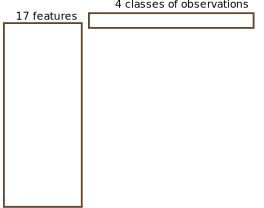
\includegraphics[width=0.7\linewidth]{pca-features-observations}

        Same question: what linear combination of features maximize the
        variance in the dataset? $\Rightarrow$ PCA!
    \end{center}
    }

    \only<4->{

    \begin{columns}
        \begin{column}{0.5\linewidth}
    \begin{center}
        \includegraphics[width=\linewidth]{pca-food-example}
    \end{center}

            \only<6>{
                \small $pc_1 \approx 0.4 \times \text{potatoes} + 0.2 \times
                \text{softs} - 0.4 \times \text{alcohol} - 0.6 \times \text{fruits}$
            }

        \end{column}
        \begin{column}{0.5\linewidth}
            \begin{center}
                \includegraphics[width=\linewidth]{pca-food-example-1-eigenvector}

                \includegraphics<5->[width=\linewidth]{pca-food-example-2-eigenvector}

                \includegraphics<6->[width=\linewidth]{pca-food-example-load-plot}
            \end{center}
        \end{column}
    \end{columns}
    \only<4>{
        \small
        The \emph{first principal component} \texttt{pc1} is the best possible linear
        combination. Can you guess what it is?
    }
    \only<5>{
        \small
        We can add more principal components to better \emph{explain the dataset
        variance}. From a classification perspective, 2 components seem
        sufficient to separate our 4 nations: We can \textbf{reduce} our 17 dimensions to
        only 2
    }

    }

\end{frame}
}

%\imageframe[scale=0.9, caption={Applied to handwriting}]{pca}
%\videoframe{figs/face_recognition/cowriter.mp4?start=135}

\imageframe[scale=0.9, caption={Applied to faces}]{dataset}

{
    \paper{\source{https://github.com/bytefish/facerecognition_guide}{Philipp
    Wagner, Face Recognition with Python} (code source available as well)}

\begin{frame}{PCA Algorithm}
    Let $\mathbf{X} = \{ \mathbf{x}_{1}, \mathbf{x}_{2}, \ldots, \mathbf{x}_{n} \}$ be a vector with observations $\mathbf{x}_i \in \mathbb{R}^{d}$.

    \begin{enumerate}
        \item Compute the mean $\mu$
            \[
                \mu = \frac{1}{n} \sum_{i=1}^{n} \mathbf{x}_{i}
            \]
        \item Compute the the Covariance Matrix $S$
            \[
                S = \frac{1}{n} \sum_{i=1}^{n} (\mathbf{x}_{i} - \mu) (\mathbf{x}_{i} - \mu)^{T}
            \]
        \item Compute the eigenvalues $\lambda_{i}$ and eigenvectors $\mathbf{v}_{i}$ of $S$
            \[
                S \cdot \mathbf{v}_{i} = \lambda_{i} \mathbf{v}_{i} \text{\hspace{1em} with } i=1,2,\ldots,n
            \]
        \item Order the eigenvectors descending by their eigenvalue. The $k$
            principal components are the eigenvectors corresponding to the $k$
            largest eigenvalues.

    \end{enumerate}

\end{frame}
}


\begin{frame}[fragile]{Python code}

\begin{pythoncode}
def pca(X):

    mu = X.mean(axis=0)
    X = X - mu
    C = np.dot(X.T,X)
    eigenvalues, eigenvectors = np.linalg.eigh(C)

    # sort eigenvectors descending by their eigenvalue
    idx = np.argsort(-eigenvalues)
    eigenvalues = eigenvalues[idx]
    eigenvectors = eigenvectors[:,idx]
    return eigenvalues, eigenvectors, mu

# D: eigenvalues, W: eigenvectors, mu: mean, X: 40 X 10304 image array
D, W, mu = pca(X) 

# plot the first 16 'eigenfaces'
images = []
for i in range(16):
    image = W[:,i].reshape(X[0].shape)
    images.append(normalize(image,0,255))

subplot(title="Eigenfaces", images=images, rows=4, cols=4)

\end{pythoncode}
\end{frame}


\imageframe{dataset}
\imageframe{eigenfaces}

\begin{frame}{PCA Projection and Reconstruction}

    The $k$ principal components of an observed vector
    $\mathbf{x}\bubblemark{image}$ are then given by:

    \[
        \mathbf{y} = W^{T} (\mathbf{x} - \mu)
    \]

    where $W\bubblemark{pcabasis} = (\mathbf{v}_{1}, \mathbf{v}_{2}, \ldots, \mathbf{v}_{k})$.
    
    \bubble<1->[80][0.5][3cm]{image}{The image of a face!}
    \bubble<1->[100]{pcabasis}{The PCA basis}

\end{frame}

\imageframe[scale=0.8]{pca-projections-1}
\imageframe[scale=0.8]{pca-projections-2}
\imageframe[scale=0.8]{pca-projections-3}

\begin{frame}{PCA Projection and reconstruction}

    The $k$ principal components of an observed vector
    $\mathbf{x}\bubblemark{image}$ are then given by:

    \[
        \mathbf{y} = W^{T} (\mathbf{x} - \mu)
    \]

    where $W\bubblemark{pcabasis} = (\mathbf{v}_{1}, \mathbf{v}_{2}, \ldots,
    \mathbf{v}_{k})$. $\mathbf{y}$ is the \textbf{projection} of $\mathbf{x}$
    onto
    $W$.
    
    \bubble<1->[80][0.5][3cm]{image}{The image of a face!}
    \bubble<1->[100]{pcabasis}{The PCA basis}


    The reconstruction from the PCA basis is given by:

    \[
        \mathbf{x} = W \cdot \mathbf{y} + \mu
    \]

\end{frame}

\begin{frame}[fragile]{Python code}

\begin{pythoncode}
def project(W, X, mu=None):
    if mu is None:
        return np.dot(X,W)
    return np.dot(X - mu, W)

def reconstruct(W, Y, mu=None):
    if mu is None:
        return np.dot(Y,W.T)
    return np.dot(Y, W.T) + mu

images = []
for nb_evs in range(10, 310, 20):
    P = project(W[:,0:nb_evs], X[0].reshape(1,-1), mu)
    R = reconstruct(W[:,0:nb_evs], P, mu)

    R = R.reshape(X[0].shape)
    images.append(normalize(R,0,255))

subplot(title="Reconstruction of one face", images=images, rows=4, cols=4)
\end{pythoncode}
\end{frame}

\imageframe{one-face}

\begin{frame}{Why is it useful?}


    Original images: $dim(\mathbf{x}) = 92 \times 112 = 10304$ pixels: large number of dimensions!

    $\Rightarrow$ difficult to tell whether 2 images represent the same person
    (\ie \emph{classify} them).

    \pause

    With the PCA, we project our test image onto a PCA basis of $k$ principal
    components: $\mathbf{y} = W^{T} (\mathbf{x} - \mu)$ with $W = (\mathbf{v}_{1}, \mathbf{v}_{2}, \ldots, \mathbf{v}_{k})$.


    $dim(\mathbf{y}) = k$ can typically be much smaller than $dim(\mathbf{x})$

    \pause

    \textbf{We effectively ``summarize'' our image into a few key values}, along
    the principal axes of variation of our dataset.

    $\Rightarrow$ these values discriminate effectively amongst our images
    (maximise variance)
    
    $\Rightarrow$ \textbf{Well suited for classification!}

\end{frame}

\imageframe{reconstruction-1-eigenfaces}
\imageframe{reconstruction-10-eigenfaces}
\imageframe{reconstruction-50-eigenfaces}

\begin{frame}{}
    \begin{center}
        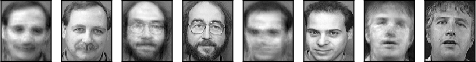
\includegraphics[width=\linewidth]{reconstruction-50-eigenfaces-top-row}

        \vspace{2em}
        Remember: these faces are reconstructed from 50 values (to be compared
        to the 10304 values required for the original photos).

        \vspace{2em}

        \pause

        PCA is often used as a \textbf{dimensionality reduction} technique (\ie a
        kind of data lossy data compression).

    \end{center}
\end{frame}


\section[Face recognition]{Face recognition}

\imageframe{face-recognition-challenge}

\imageframe[scale=0.8]{pca-projections-4}
\imageframe[scale=0.8]{pca-projections-5}
\imageframe[scale=0.8]{pca-projections-6}

\begin{frame}{Recognition}

    \begin{enumerate}
        \item \textbf{learn a model} by (1) computing the PCA basis of the
            training set, (2) projecting each training face onto that basis
        \item \textbf{project the test image} (eg, the face you want to
            recognise)
        \item \textbf{find the 1-nearest neighbour}
    \end{enumerate}
\end{frame}

\begin{frame}[fragile]{Python code}


    \begin{columns}
        \begin{column}{0.5\linewidth}
\begin{minted}[fontsize=\scriptsize]{python}
def dist(p, q):
    p = np.asarray(p).flatten()
    q = np.asarray(q).flatten()
    return np.sqrt(np.sum(
                    np.power((p-q),2)
                    ))


def learn_model(X):
    # compute PCA basis
    D, W, mu = pca(X, nb_evs=10)
    # compute projections
    projections = []
    for xi in X:
        yi = project(W,
                   xi.reshape(1,-1), 
                   mu)
        projections.append(yi)

    return W, projections
\end{minted}

        \end{column}
        \begin{column}{0.5\linewidth}


\begin{minted}[fontsize=\scriptsize]{python}
def predict(x, W, projections):
    minDist = np.finfo('float').max
    minClass = -1
    Q = project(W, x.reshape(1,-1), mu)

    for i in range(len(projections)):
        dist = dist(projections[i], Q)
        if dist < minDist:
            minDist = dist
            faceClass = faceClasses[i]
    return faceClass


X, faceClasses = read_images()
W, projections = learn_model(X)
predict(test_image, W, projections)

\end{minted}
        \end{column}
    \end{columns}

\end{frame}


%%%%%%%%%%%%%%%%%%%%%%%%%%%%%%%%%%%%%%%%%%%%%%%%%%%%%%%%%%%%%%%%%%%%%%%%%%%%%%%%
\section{From social signal to internal state}

\begin{frame}{From social signal to internal state}

    Question: can we infer the internal state of the children based on either
    image?

    \begin{center}
        \includegraphics[width=0.9\linewidth]{pinsoro-kinematics/clips}
    \end{center}

\end{frame}

{
    \paper{Lemaignan et al. {\bf The PInSoRo
    dataset: Supporting the data-driven study of child-child...} PLOS One 2018}
\begin{frame}{13000+ annotations}
    \begin{center}
        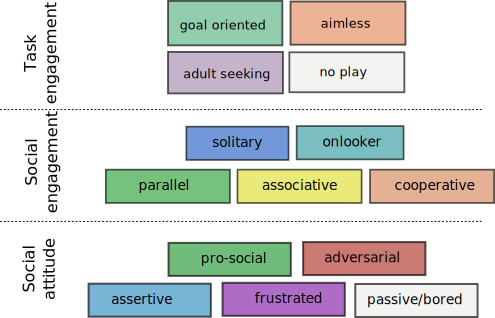
\includegraphics[width=0.8\linewidth]{pinsoro-kinematics/coding-scheme}
    \end{center}
\end{frame}
}
\videoframe[0.56]{figs/pinsoro-kinematics/annotations.mp4?autostart}
\videoframe[0.56]{figs/pinsoro-kinematics/pinsoro-matplotlib.mp4?autostart}

{
    \paper{Bartlett, Edmunds, Belpaeme, Thill, Lemaignan, \textbf{What Can You
    See? Identifying Cues on Internal States...}, FrontiersIn 2019}
\begin{frame}{}
    \begin{itemize}
        \item 20 clips extracted from the dataset, featuring notable social
            behaviours (boredom, aggression, cooperation, dominance, fun,
            excitement)
        \item online study to ask people to annotate the clips along 20
            dimensions
    \end{itemize}
\end{frame}
}

\imageframe[caption={200 participants, 4 clips each, on MTurk}]{kinematics_social_dynamics/questionnaire.png}


%%%%%%%%%%%%%%%%%%%%%%%%%%%%%%%%%%%%%%%%%%%%%%%%%%%%%%%%%%%%%%%%%%%%%%%%%%%%%%%%
%%%%%%%%%%%%%%%%%%%%%%%%%%%%%%%%%%%%%%%%%%%%%%%%%%%%%%%%%%%%%%%%%%%%%%%%%%%%%%%%
%%%%%%%%%%%%%%%%%%%%%%%%%%%%%%%%%%%%%%%%%%%%%%%%%%%%%%%%%%%%%%%%%%%%%%%%%%%%%%%%

\miniframesoff

\begin{frame}{We've barely scratched the surface!}

\only<1>{
Social signal processing is about extracting relevant information from the
social environment.

Some techniques work relatively well:

\begin{itemize}

\item Face recognition, voice activity detection, gender
  classification, \ldots{}
\end{itemize}

Some work, but need improvement:

\begin{itemize}

\item Gaze detection, basic emotion recognition, speech recognition, \ldots{}
\end{itemize}
}

\only<2>{
But many open problems remain, eg:

\begin{itemize}

\item Complex real-word affect and emotion recognition (e.g.~embarrassment,
  pride).
\item Speech recognition for atypical speakers (children, elderly),
  multi-party interaction, \ldots{}
\item most body language
\item group dynamics
\end{itemize}
}

\end{frame}



\begin{frame}{}
    \begin{center}
        \Large
        That's all for today, folks!\\[2em]
        \normalsize
        Questions:\\
        \url{severin.lemaignan@brl.ac.uk} \\[1em]

        Slides:\\ \href{https://github.com/severin-lemaignan/lecture-social-signal-processing}{\small github.com/severin-lemaignan/lecture-social-signal-processing}

    \end{center}
\end{frame}


\begin{frame}{Classification of auditory signals}

    Raw signals will in most cases require pre-processing to extract
features.

The raw social signal (audio or video) requires pre-processing\bubblemark{preprocessing} to
extract between 10 and over a 1000 \textbf{features}.

\begin{itemize}

    \item A raw signals contains too much data, and cannot be fed to the
      classifier immediately.

        \begin{center}
            \includegraphics[width=0.5\linewidth]{rawaudio}
        \end{center}

    \item Pre-processing extracts feature data which is relevant for the
  information which we are after (pitch, volume/energy, duration,
  formant frequencies, \ldots{})
    \item These features then form the input for the classifier.
\end{itemize}

    {\footnotesize
For more information see, for example, Liang et al. (2005)
\href{http://ieeexplore.ieee.org/xpls/icp.jsp?arnumber=1571239}{Feature
analysis and extraction for audio automatic classification}, Systems,
Man and Cybernetics, 2005 IEEE International Conference on.
    }

\bubble<2>[50][0.7][5cm]{preprocessing}{An exception to this are Convolutional Neural
    Networks, which can deal with unprocessed data}

\end{frame}

\begin{frame}{Example: recognising gender from speech}

Can we automatically recognise someone's gender from speech?

3,168 recorded voice samples, collected from male and female speakers.

\begin{itemize}

\item Examples from the database: male (US), female (US), male (Scotish)
\end{itemize}

    \begin{center}
    \audio{figs/male-us.mp4}\hspace{0.3em}
    \audio{figs/male-scottish.mp4}\hspace{0.3em}
    \audio{figs/female-us.mp4}
    \end{center}


The voice samples are pre-processed by acoustic analysis in R using the
{\tt seewave}, {\tt warbleR} and {\tt tuneR} packages, with an analysed frequency range of
0hz-280Hz (fundamental frequency of human speech).


\source{https://www.kaggle.com/primaryobjects/voicegender}{data and more information}


\end{frame}

\begin{frame}{The 20 features used for gender classification}

    \only<1>{
\begin{itemize}

\item \textbf{meanfreq}: mean frequency (in kHz)
\item \textbf{sd}: standard deviation of frequency
\item \textbf{median}: median frequency (in kHz)
\item \textbf{Q25}: first quantile (in kHz)
\item \textbf{Q75}: third quantile (in kHz)
\item \textbf{IQR}: interquantile range (in kHz)
\item \textbf{skew}: skewness (see note in specprop description)
\item \textbf{kurt}: kurtosis (see note in specprop description)
\item \textbf{sp.ent}: spectral entropy
\item \textbf{sfm}: spectral flatness
\item \textbf{mode}: mode frequency
\item \textbf{centroid}: frequency centroid (see specprop)
\item \textbf{peakf}: peak frequency (frequency with highest energy)
\item \textbf{meanfun}: average of fundamental frequency measured across
  acoustic signal
\end{itemize}
}
    \only<2>{
\begin{itemize}

\item \textbf{minfun}: minimum fundamental frequency measured across
  acoustic signal
\item \textbf{maxfun}: maximum fundamental frequency measured across
  acoustic signal
\item \textbf{meandom}: average of dominant frequency measured across
  acoustic signal
\item \textbf{mindom}: minimum of dominant frequency measured across
  acoustic signal
\item \textbf{maxdom}: maximum of dominant frequency measured across
  acoustic signal
\item \textbf{dfrange}: range of dominant frequency measured across acoustic
  signal
\item \textbf{modindx}: modulation index. Calculated as the accumulated
  absolute difference between adjacent measurements of fundamental
  frequencies divided by the frequency range
\end{itemize}
}

\end{frame}

\begin{frame}{Example: recognising gender from speech}

    \begin{center}
        \includegraphics[width=\linewidth]{vector-gender-voice}
    \end{center}
\end{frame}

\begin{frame}{Example: recognising gender from speech}

Performance

\begin{itemize}

\item kNN (k = 7): 97.8\% classified correctly.
\item SVM: 97.5\% classified correctly.
\end{itemize}

Recognising gender from speech is easy and robust.

All classification algorithms can deal with this problem.

\end{frame}


\end{document}
